%%%%%%%%%%%%%%%%%%%%%%%%%%%%%%%%%%%%%%%%%%%%%%%%%%%%%%%%%%%%%%%%%
\chapter{TABLES AND FIGURES}\label{CH2}
%%%%%%%%%%%%%%%%%%%%%%%%%%%%%%%%%%%%%%%%%%%%%%%%%%%%%%%%%%%%%%%%%

\vspace{-12pt} %iki başlık alt alta. iki katı boşluk olmasın

\section{Figure Citations and Figure Example}

Tables and figures given in appendices must be numbered with the number of the appendix they are in (i.e. \textbf{Table A.1}, \textbf{Table A.2}, \textbf{Figure A.1}, \textbf{Figure A.2}).

In tables and figures, font size could be reduced to 8 pt, if necessary.

Tables must be prepared using the same font type as the thesis. The font type used in figures must be consistent throughout the thesis.

Tables and figures must be placed after they are first cited in the main text body, but must be as close as possible, in accordance with the rules in this guideline such as \figurename\ \ref{fig:ch2-1}. All tables and figures must be cited before they are used in the main text body.

All tables and figures must be horizontally centered on the page.

\vspace{6pt} % 12pt
\begin{figure}[!ht]
    \centering
    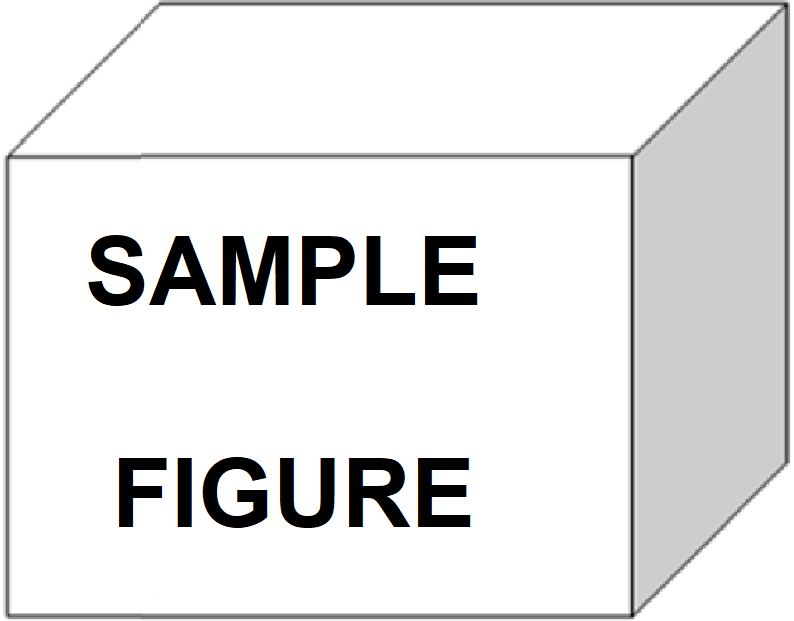
\includegraphics[width=5cm,keepaspectratio=true]{./fig/sekil1.png}
    % sekil2.eps: 0x0 pixel, 300dpi, 0.00x0.00 cm, bb=14 14 818 556
    \caption{All tables and figures must be horizontally centered on the page.}
    \label{fig:ch2-1}
\end{figure}
\vspace{-9pt} % 12pt 

The numbering of the tables and the figures must be such that the first number is the number of the chapter the table/figure is placed under (for appendices, the letter of the appendix), and the second number is the number of order (i.e. Table 1.2, Figure 3.5, Table A.1, Figure B.5). The words “Table” and “Figure” and numbers must be bold.

For table numbers and captions, 1 line spacing, 12 pt (before) and 6 pt (after) paragraph spacing must be set. Table captions must be ended with a full stop. A table and its caption must be on the same page. 

Multiple tables/figures could be placed on one page, however, table/figures spanning more than 4 consecutive pages must be given in appendices rather than the main text body.

The first paragraph following a table must have 12 pt (before) and 6 pt (after) paragraph spacing. Titles following a table must have the standard formatting as previously specified. 

Footnotes for a table must be written with 1 line spacing and a font size 2 pt smaller than the main text body. 

For figure numbers and captions, 1 line spacing, 6 pt (before) and 12 pt (after) paragraph spacing must be set. Figure captions must be ended with a full stop. A figure and its caption must be on the same page. 

For figures spanning more than one page, the same number and caption must be written below the continued figure, with the expression ”continued” added in brackets (i.e. \textbf{Table 1.1 (continued):} Metal composition of wastes. \textbf{Figure 1.1 (continued):} Water supply network of ISTANBUL.).

Plots, images and musical notes must be numbered and captioned as figures. Musical notes must be written according to the format rules set by the İTU School of Traditional Turkish Music. 

It is recommended that elements that increase the page thickness and disrupt the binding structure of theses such as  folded pages or additional items embedded on pages are given as appendices.

\figurename\ \ref{fig:ch2-2} Sed diam nonumy eirmod tempor invidunt ut labore et dolore magna aliquyam erat, sed diam voluptua. At vero eos et accusam et justo duo dolores et ea rebum. Lorem ipsum dolor sit amet, consetetur sadipscing elitr, sed diam nonumy eirmod tempor invidunt ut labore et dolore magna aliquyam erat, sed diam voluptua. At vero eos et accusam et justo duo dolores et ea rebum. At vero eos et accusam et justo duo dolores et ea rebum. At vero eos et accusam et justo duo dolores et ea rebum. At vero eos et accusam et justo duo dolores et ea rebum. At vero eos et accusam et justo duo dolores et ea rebum. At vero eos et accusam et justo duo dolores et ea rebum. At vero eos et accusam et justo duo dolores et ea rebum.

Lorem ipsum dolor sit amet, consetetur sadipscing elitr, sed diam nonumy eirmod tempor invidunt ut labore et dolore magna aliquyam erat, sed diam voluptua. At vero eos et accusam et justo duo dolores et ea rebum. At vero eos et accusam et justo duo dolores et ea rebum. At vero eos et accusam et justo duo dolores et ea rebum.

\vspace{6pt} % 12pt
\begin{figure}[!ht]
    \centering
    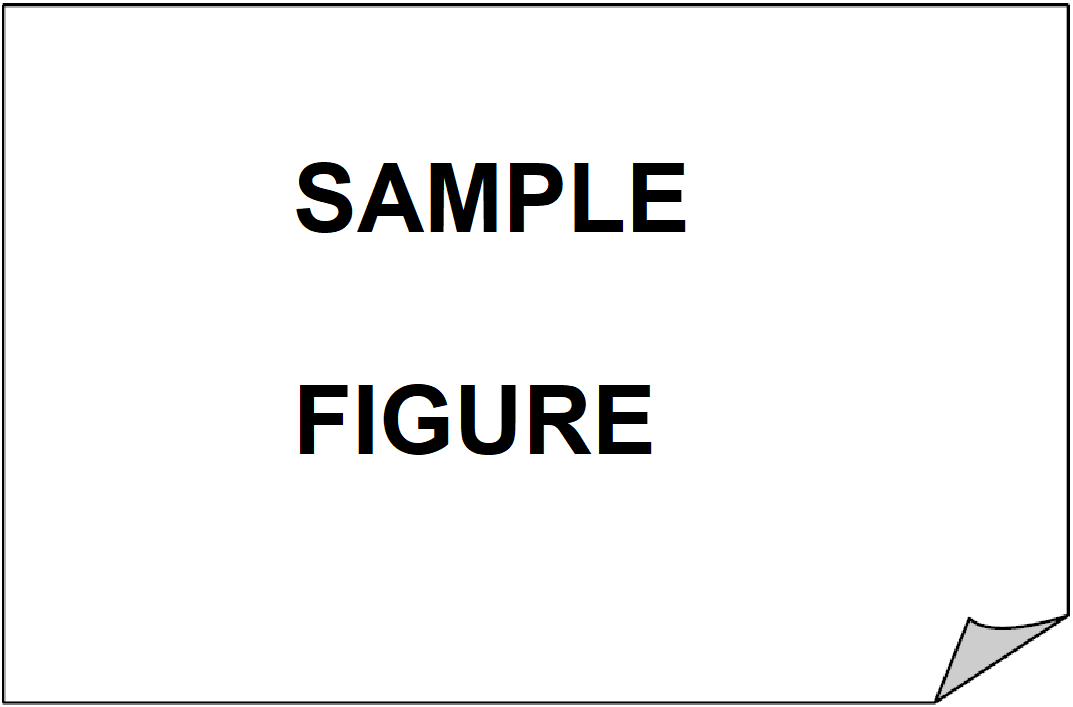
\includegraphics[width=10cm,keepaspectratio=true]{./fig/sekil2.png}
    % sekil2.eps: 0x0 pixel, 300dpi, 0.00x0.00 cm, bb=14 14 818 556
    \caption{Example figure.}
    \label{fig:ch2-2}
\end{figure}
\vspace{-9pt} % 12pt 

\section{Landscape-oriented, full-page figure}

Lorem ipsum dolor sit amet, consetetur sadipscing elitr, sed diam nonumy eirmod tempor invidunt ut labore et dolore magna aliquyam erat, sed diam voluptua. At vero eos et accusam et justo duo dolores et ea rebum (\figurename\ \ref{fig:ch2-3}). Lorem ipsum dolor sit amet, consetetur sadipscing elitr, sed diam nonumy eirmod tempor invidunt ut labore et dolore magna aliquyam erat, sed diam voluptua. At vero eos et accusam et justo duo dolores et ea rebum. 
Lorem ipsum dolor sit amet, consetetur sadipscing elitr, sed diam nonumy eirmod tempor invidunt ut labore et dolore magna aliquyam erat, sed diam voluptua. At vero eos et accusam et justo duo dolores et ea rebum. Lorem ipsum dolor sit amet, consetetur sadipscing elitr, sed diam nonumy eirmod tempor invidunt ut labore et dolore magna aliquyam erat, sed diam voluptua. At vero eos et accusam et justo duo dolores et ea rebum. Lorem ipsum dolor sit amet, consetetur sadipscing elitr, sed diam nonumy eirmod tempor invidunt ut labore et dolore magna aliquyam erat, sed diam voluptua. At vero eos et accusam et justo duo dolores et ea rebum.   

\begin{landscape}
\thispagestyle{empty}
\vspace{6pt}
\begin{figure}[htp!]
      \centering
      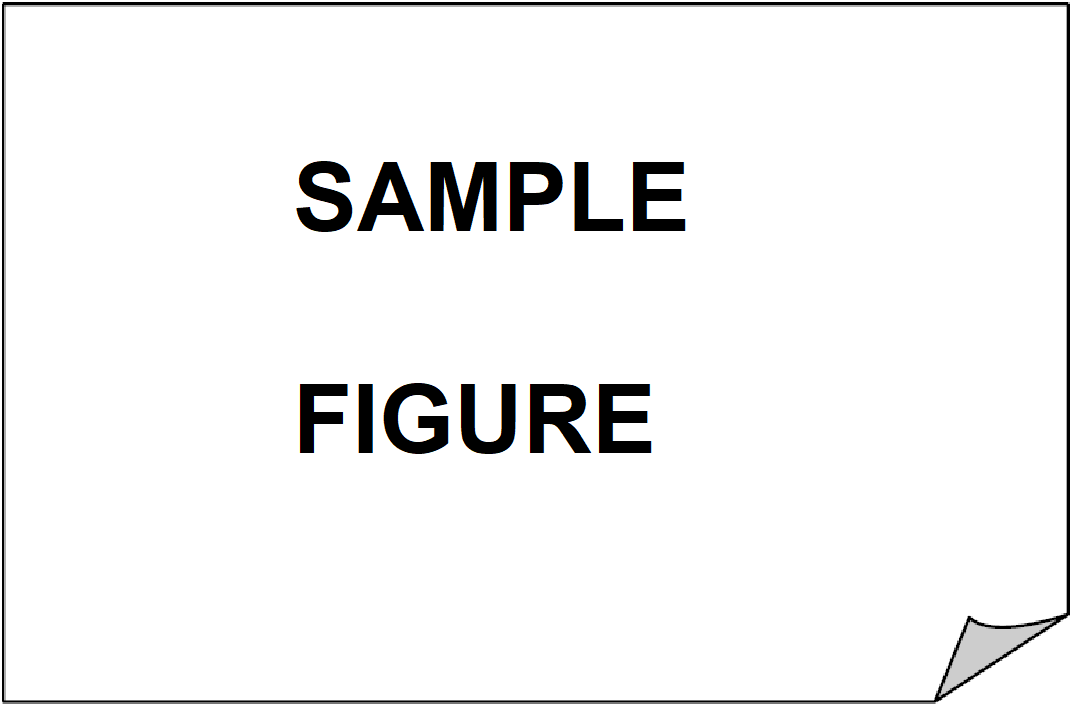
\includegraphics[width=500pt,keepaspectratio=true]{./fig/sekil3.png}
      % sekil3.eps: 0x0 pixel, 300dpi, 0.00x0.00 cm, bb=14 14 1155 740
      \caption{Landscape-oriented, full-page figure.}    
      \label{fig:ch2-3}
\end{figure}
\vspace{-6pt}
\vfill\hbox{ }

\ifodd\value{page} % Tek sf
\begin{textblock*}{1cm}[0,0](19.5cm,14.85cm) % 210 - 15
\else		% Cift sf
\begin{textblock*}{1cm}[0,0](18.0cm,14.85cm) % 210 - 30
\fi
{\rotatebox{90}{\centering\thepage}} % sf numarası
\end{textblock*}
\end{landscape}

Lorem ipsum dolor sit amet, consetetur sadipscing elitr, sed diam nonumy eirmod tempor invidunt ut labore et dolore magna aliquyam erat, sed diam voluptua. At vero eos et accusam et justo duo dolores et ea rebum. Lorem ipsum dolor sit amet, consetetur sadipscing elitr, sed diam nonumy eirmod tempor invidunt ut labore et dolore magna aliquyam erat, sed diam voluptua. At vero eos et accusam et justo duo dolores et ea rebum. Lorem ipsum dolor sit amet, consetetur sadipscing elitr, sed diam nonumy eirmod tempor invidunt ut labore et dolore magna aliquyam erat, sed diam voluptua. At vero eos et accusam et justo duo dolores et ea rebum. Lorem ipsum dolor sit amet, consetetur sadipscing elitr, sed diam nonumy eirmod tempor invidunt ut labore et dolore magna aliquyam erat, sed diam voluptua. At vero eos et accusam et justo duo dolores et ea rebum.

\section{Table Citations and Table Example}

Lorem ipsum dolor sit amet, consetetur sadipscing elitr, sed diam nonumy eirmod tempor invidunt ut labore et dolore magna aliquyam erat, sed diam voluptua. At vero eos et accusam et justo duo dolores et ea rebum. Stet clita kasd gub rgren, no sea takimata sanctus est Lorem ipsum dolor sit amet, consetetur sadipscing elitr, sed diam nonumy eirmod tempor invidunt ut lab ore sit et dolore magna.

As seen in \tablename\ \ref{table:ch2-1} lorem ipsum dolor sit amet, consetetur sadipscing elitr, sed diam nonumy eirmod tempor invidunt ut labore et dolore magna aliquyam erat, sed diam voluptua. At vero eos et accusam et justo duo dolores et ea rebum. Stet clita kasd gub rgren, no sea takimata sanctus est Lorem ipsum dolor sit amet, consetetur sadipscing elitr, sed diam nonumy eirmod tempor invidunt ut lab ore sit et dolore magna.

\vspace{6pt} % 12pt
\begin{table}[!ht]
\centering
\setlength{\tabcolsep}{14pt}
\caption{Table captions must be ended with a full stop.}
\begin{tabular}{cccc}
\toprule\midrule
Column A & Column B & Column C & Column D \\
\midrule
Row A & Row A & Row A & Row A \\
Row B & Row B & Row B & Row B \\
Row C & Row C & Row C & Row C \\
\bottomrule
\end{tabular}
\label{table:ch2-1}
\end{table}
\vspace{-9pt} % 12pt 

Lorem ipsum dolor sit amet, consetetur sadipscing elitr, sed diam nonumy eirmod tempor invidunt ut labore et dolore magna aliquyam erat, sed diam voluptua. At vero eos et accusam et justo duo dolores et ea rebum. 

Lorem ipsum dolor sit amet, consetetur sadipscing elitr, sed diam nonumy eirmod tempor invidunt ut labore et dolore magna aliquyam erat, sed diam voluptua. At vero eos et accusam et justo duo dolores et ea rebum. Stet clita kasd gub rgren, no sea takimata sanctus est Lorem ipsum dolor sit amet, consetetur sadipscing elitr, sed diam nonumy eirmod tempor invidunt ut lab ore sit et dolore magna. Lorem ipsum dolor sit amet, consetetur sadipscing elitr, sed diam nonumy eirmod tempor invidunt ut labore et dolore magna aliquyam erat, sed diam voluptua. At vero eos et accusam et justo duo dolores et ea rebum \tablename\ \ref{table:ch2-2}.

\vspace{6pt} % 12pt
\begin{table}[!ht]
\centering
\setlength{\tabcolsep}{14pt}
\caption{Table captions must be ended with a full stop.}
\begin{tabular}{cccc}
\toprule\midrule
Column A & Column B & Column C & Column D \\
\midrule
Row A & Row A & Row A & Row A \\
Row B & Row B & Row B & Row B \\
Row C & Row C & Row C & Row C \\
\bottomrule
\end{tabular}
\label{table:ch2-2}
\end{table}
\vspace{-9pt} % 12pt 

Lorem ipsum dolor sit amet, consetetur sadipscing elitr, sed diam nonumy eirmod tempor invidunt ut labore et dolore magna aliquyam erat, sed diam voluptua. At vero eos et accusam et justo duo dolores et ea rebum. Stet clita kasd gub rgren, no sea takimata sanctus est Lorem ipsum dolor sit amet, consetetur sadipscing elitr, sed diam nonumy eirmod tempor invidunt ut lab ore sit et dolore magna. Lorem ipsum dolor sit amet, consetetur sadipscing elitr, sed diam nonumy eirmod tempor invidunt ut labore et dolore magna aliquyam erat, sed diam voluptua. At vero eos et accusam et justo duo dolores et ea rebum. 

\section{Landscape-oriented, full-page table}

Lorem ipsum dolor sit amet, consetetur sadipscing elitr, sed diam nonumy eirmod tempor invidunt ut labore et dolore magna aliquyam erat, sed diam voluptua. At vero eos et accusam et justo duo dolores et ea rebum. Stet clita kasd gub rgren, no sea takimata sanctus est Lorem ipsum dolor sit amet, consetetur sadipscing elitr, sed diam nonumy eirmod tempor invidunt ut lab ore sit et dolore magna \tablename\ \ref{table:ch2-3}.

\begin{landscape}
\thispagestyle{empty}
\vspace{6pt} % 12pt
\begin{table}[htp]
\centering
\setlength{\tabcolsep}{14pt}
\captionsetup{justification=centerlast}
\caption{Captioning in landscape-oriented pages: the most important aspect is to align the lines horizontally. lorem ipsum dolor sit amet, consetetu.}
\label{table:ch2-3}
\begin{tabular}{lccrrrrr}
\toprule\midrule
\multirow{2}{*}{Parametre} & \multirow{2}{*}{Column 2} & \multirow{2}{*}{Column 3} & \multicolumn{3}{c}{Column 4} & \multicolumn{2}{c}{Column 5}\\ \cmidrule(lr){4-6} \cmidrule(lr){7-8}
  & & & Subcolumn & Subcolumn & Subcolumn & Subcolumn & Subcolumn\\
\midrule
Row 1 & -7.680442 & 7.6986348 & 0.00 & 0.00 & 0.00 & 12 & 12 \\
Row 2 & 140 & - & 0.50 & 0.00 & 0.00 & 0 & 0 \\
Row 3 & 37.174357 & 37.16192697 & 0.00 & 0.00 & 0.00 & 0 & 24 \\
Row 4 & 140 & - & 0.50 & 0.00 & 0.00 & 0 & 0 \\
Row 5 & 37.174357 & 37.16192697 & 0.00 & 0.00 & 0.00 & 0 & 24 \\
Row 6 & 140 & - & 0.50 & 0.00 & 0.00 & 0 & 0 \\
Row 7 & 37.174357 & 37.16192697 & 0.00 & 0.00 & 0.00 & 0 & 24 \\
Row 8 & 140 & - & 0.50 & 0.00 & 0.00 & 0 & 0 \\
Row 9 & 37.174357 & 37.16192697 & 0.00 & 0.00 & 0.00 & 0 & 24 \\
Row 10 & 140 & - & 0.50 & 0.00 & 0.00 & 0 & 0 \\
Row 11 & 37.174357 & 37.16192697 & 0.00 & 0.00 & 0.00 & 0 & 24 \\
Row 12 & 140 & - & 0.50 & 0.00 & 0.00 & 0 & 0 \\
Row 13 & 37.174357 & 37.16192697 & 0.00 & 0.00 & 0.00 & 0 & 24 \\
Row 14 & 140 & - & 0.50 & 0.00 & 0.00 & 0 & 0 \\
Row 15 & 37.174357 & 37.16192697 & 0.00 & 0.00 & 0.00 & 0 & 24 \\
\bottomrule
\end{tabular}
\end{table}
\vspace{-9pt} % 12pt 
\vfill\hbox{ }

\ifodd\value{page} % Tek sf
\begin{textblock*}{1cm}[0,0](19.5cm,14.85cm) % 210 - 15
\else		% Cift sf
\begin{textblock*}{1cm}[0,0](18.0cm,14.85cm) % 210 - 30
\fi
{\rotatebox{90}{\centering\thepage}} % sf numarası
\end{textblock*}
\end{landscape}

\begin{landscape}
\thispagestyle{empty}
\vspace{6pt} % 12pt
\begin{table}[htp]
\centering
\setlength{\tabcolsep}{14pt}
\captionsetup{justification=centerlast}
\caption*{\textbf{\tablename\ \ref{table:ch2-3} (continued) : } Captioning in landscape-oriented pages: the most important aspect is to align the lines horizontally. lorem ipsum dolor sit amet, consetetu.}
\begin{tabular}{lccrrrrr}
\toprule\midrule
\multirow{2}{*}{Parametre} & \multirow{2}{*}{Column 2} & \multirow{2}{*}{Column 3} & \multicolumn{3}{c}{Column 4} & \multicolumn{2}{c}{Column 5}\\ \cmidrule(lr){4-6} \cmidrule(lr){7-8}
  & & & Subcolumn & Subcolumn & Subcolumn & Subcolumn & Subcolumn\\
\midrule
Row 1 & -7.680442 & 7.6986348 & 0.00 & 0.00 & 0.00 & 12 & 12 \\
Row 2 & 140 & - & 0.50 & 0.00 & 0.00 & 0 & 0 \\
Row 3 & 37.174357 & 37.16192697 & 0.00 & 0.00 & 0.00 & 0 & 24 \\
Row 4 & 140 & - & 0.50 & 0.00 & 0.00 & 0 & 0 \\
Row 5 & 37.174357 & 37.16192697 & 0.00 & 0.00 & 0.00 & 0 & 24 \\
Row 6 & 140 & - & 0.50 & 0.00 & 0.00 & 0 & 0 \\
Row 7 & 37.174357 & 37.16192697 & 0.00 & 0.00 & 0.00 & 0 & 24 \\
Row 8 & 140 & - & 0.50 & 0.00 & 0.00 & 0 & 0 \\
Row 9 & 37.174357 & 37.16192697 & 0.00 & 0.00 & 0.00 & 0 & 24 \\
Row 10 & 140 & - & 0.50 & 0.00 & 0.00 & 0 & 0 \\
Row 11 & 37.174357 & 37.16192697 & 0.00 & 0.00 & 0.00 & 0 & 24 \\
Row 12 & 140 & - & 0.50 & 0.00 & 0.00 & 0 & 0 \\
Row 13 & 37.174357 & 37.16192697 & 0.00 & 0.00 & 0.00 & 0 & 24 \\
Row 14 & 140 & - & 0.50 & 0.00 & 0.00 & 0 & 0 \\
Row 15 & 37.174357 & 37.16192697 & 0.00 & 0.00 & 0.00 & 0 & 24 \\
\bottomrule
\end{tabular}
\end{table}
\vspace{-9pt} % 12pt 
\vfill\hbox{ }

\ifodd\value{page} % Tek sf
\begin{textblock*}{1cm}[0,0](19.5cm,14.85cm) % 210 - 15
\else		% Cift sf
\begin{textblock*}{1cm}[0,0](18.0cm,14.85cm) % 210 - 30
\fi
{\rotatebox{90}{\centering\thepage}} % sf numarası
\end{textblock*}
\end{landscape}

\vspace*{-\topskip}
\section{Alternative full-page long table}

Lorem ipsum dolor sit amet, consetetur sadipscing elitr, sed diam nonumy eirmod tempor invidunt ut labore et dolore magna aliquyam erat, sed diam voluptua. At vero eos et accusam et justo duo dolores et ea rebum. Lorem ipsum dolor sit amet, consetetur sadipscing elitr, sed diam nonumy eirmod tempor invidunt ut labore et dolore magna aliquyam erat, sed diam voluptua. At vero eos et accusam et justo duo dolores et ea rebum. Lorem ipsum dolor sit amet, consetetur sadipscing elitr, sed diam nonumy eirmod tempor invidunt ut labore et dolore magna aliquyam erat, sed diam voluptua. At vero eos et accusam et justo duo dolores et ea rebum \tablename\ \ref{table:ch2-4}.

\vspace{6pt} % 12pt
\begin{small}
\begin{longtable}{ccc}
		%Here is the caption, the stuff in [] is the table of contents entry,
		%the stuff in {} is the title that will appear on the first page of the
		%table.
		\caption{An example of a longtable table which is a long table.}\label{table:ch2-4}\\
		%This is the header for the first page of the table...
		\toprule\midrule
		\multicolumn{1}{c}{{Time (s)}} &
		\multicolumn{1}{c}{{Triple chosen}} &
		\multicolumn{1}{c}{{Other feasible triples}} \\
		\midrule
		\endfirsthead
		
		%This is the header for the remaining page(s) of the table...
		\caption*{\textbf{\tablename\ \thetable\ (continued) :} An example of a longtable table which is a long table.} \\ 
		\toprule \midrule
		\multicolumn{1}{c}{{Time (s)}} &
		\multicolumn{1}{c}{{Triple chosen}} &
		\multicolumn{1}{c}{{Other feasible triples}} \\
		\midrule
		\endhead
		
		%This is the footer for all pages except the last page of the table...
		%\multicolumn{3}{l}{{Continued on Next Page\ldots}} \\
		\bottomrule
		\endfoot
		
		%This is the footer for the last page of the table...
		\bottomrule
		\endlastfoot
		
		%Now the data...
		0      & (1, 11, 13725) & (1, 12, 10980), (1, 13, 8235), (2, 2, 0), (3, 1, 0) \\
		2745   & (1, 12, 10980) & (1, 13, 8235), (2, 2, 0), (2, 3, 0), (3, 1, 0) \\
		5490   & (1, 12, 13725) & (2, 2, 2745), (2, 3, 0), (3, 1, 0) \\
		8235   & (1, 12, 16470) & (1, 13, 13725), (2, 2, 2745), (2, 3, 0), (3, 1, 0) \\
		% <data removed>
		164700 & (1, 13, 13725) & (2, 2, 2745), (2, 3, 0), (3, 1, 0) \\
		0      & (1, 11, 13725) & (1, 12, 10980), (1, 13, 8235), (2, 2, 0), (3, 1, 0) \\
		2745   & (1, 12, 10980) & (1, 13, 8235), (2, 2, 0), (2, 3, 0), (3, 1, 0) \\
		5490   & (1, 12, 13725) & (2, 2, 2745), (2, 3, 0), (3, 1, 0) \\
		8235   & (1, 12, 16470) & (1, 13, 13725), (2, 2, 2745), (2, 3, 0), (3, 1, 0) \\
		% <data removed>
		164700 & (1, 13, 13725) & (2, 2, 2745), (2, 3, 0), (3, 1, 0) \\
		0      & (1, 11, 13725) & (1, 12, 10980), (1, 13, 8235), (2, 2, 0), (3, 1, 0) \\
		2745   & (1, 12, 10980) & (1, 13, 8235), (2, 2, 0), (2, 3, 0), (3, 1, 0) \\
		5490   & (1, 12, 13725) & (2, 2, 2745), (2, 3, 0), (3, 1, 0) \\
		8235   & (1, 12, 16470) & (1, 13, 13725), (2, 2, 2745), (2, 3, 0), (3, 1, 0) \\
		% <data removed>
		164700 & (1, 13, 13725) & (2, 2, 2745), (2, 3, 0), (3, 1, 0) \\
		0      & (1, 11, 13725) & (1, 12, 10980), (1, 13, 8235), (2, 2, 0), (3, 1, 0) \\
		2745   & (1, 12, 10980) & (1, 13, 8235), (2, 2, 0), (2, 3, 0), (3, 1, 0) \\
		5490   & (1, 12, 13725) & (2, 2, 2745), (2, 3, 0), (3, 1, 0) \\
		8235   & (1, 12, 16470) & (1, 13, 13725), (2, 2, 2745), (2, 3, 0), (3, 1, 0) \\
		% <data removed>
		164700 & (1, 13, 13725) & (2, 2, 2745), (2, 3, 0), (3, 1, 0) \\
		0      & (1, 11, 13725) & (1, 12, 10980), (1, 13, 8235), (2, 2, 0), (3, 1, 0) \\
		2745   & (1, 12, 10980) & (1, 13, 8235), (2, 2, 0), (2, 3, 0), (3, 1, 0) \\
		5490   & (1, 12, 13725) & (2, 2, 2745), (2, 3, 0), (3, 1, 0) \\
		8235   & (1, 12, 16470) & (1, 13, 13725), (2, 2, 2745), (2, 3, 0), (3, 1, 0) \\
		% <data removed>
		164700 & (1, 13, 13725) & (2, 2, 2745), (2, 3, 0), (3, 1, 0) \\
		0      & (1, 11, 13725) & (1, 12, 10980), (1, 13, 8235), (2, 2, 0), (3, 1, 0) \\
		2745   & (1, 12, 10980) & (1, 13, 8235), (2, 2, 0), (2, 3, 0), (3, 1, 0) \\
		5490   & (1, 12, 13725) & (2, 2, 2745), (2, 3, 0), (3, 1, 0) \\
		8235   & (1, 12, 16470) & (1, 13, 13725), (2, 2, 2745), (2, 3, 0), (3, 1, 0) \\
		% <data removed>
		164700 & (1, 13, 13725) & (2, 2, 2745), (2, 3, 0), (3, 1, 0) \\
		0      & (1, 11, 13725) & (1, 12, 10980), (1, 13, 8235), (2, 2, 0), (3, 1, 0) \\
		2745   & (1, 12, 10980) & (1, 13, 8235), (2, 2, 0), (2, 3, 0), (3, 1, 0) \\
		5490   & (1, 12, 13725) & (2, 2, 2745), (2, 3, 0), (3, 1, 0) \\
		8235   & (1, 12, 16470) & (1, 13, 13725), (2, 2, 2745), (2, 3, 0), (3, 1, 0) \\
		% <data removed>
		164700 & (1, 13, 13725) & (2, 2, 2745), (2, 3, 0), (3, 1, 0) \\
		0      & (1, 11, 13725) & (1, 12, 10980), (1, 13, 8235), (2, 2, 0), (3, 1, 0) \\
		2745   & (1, 12, 10980) & (1, 13, 8235), (2, 2, 0), (2, 3, 0), (3, 1, 0) \\
		5490   & (1, 12, 13725) & (2, 2, 2745), (2, 3, 0), (3, 1, 0) \\
		8235   & (1, 12, 16470) & (1, 13, 13725), (2, 2, 2745), (2, 3, 0), (3, 1, 0) \\
		% <data removed>
		164700 & (1, 13, 13725) & (2, 2, 2745), (2, 3, 0), (3, 1, 0) \\
		0      & (1, 11, 13725) & (1, 12, 10980), (1, 13, 8235), (2, 2, 0), (3, 1, 0) \\
		2745   & (1, 12, 10980) & (1, 13, 8235), (2, 2, 0), (2, 3, 0), (3, 1, 0) \\
		5490   & (1, 12, 13725) & (2, 2, 2745), (2, 3, 0), (3, 1, 0) \\
		8235   & (1, 12, 16470) & (1, 13, 13725), (2, 2, 2745), (2, 3, 0), (3, 1, 0) \\
		% <data removed>
		164700 & (1, 13, 13725) & (2, 2, 2745), (2, 3, 0), (3, 1, 0) \\
		0      & (1, 11, 13725) & (1, 12, 10980), (1, 13, 8235), (2, 2, 0), (3, 1, 0) \\
		2745   & (1, 12, 10980) & (1, 13, 8235), (2, 2, 0), (2, 3, 0), (3, 1, 0) \\
		5490   & (1, 12, 13725) & (2, 2, 2745), (2, 3, 0), (3, 1, 0) \\
		8235   & (1, 12, 16470) & (1, 13, 13725), (2, 2, 2745), (2, 3, 0), (3, 1, 0) \\
		% <data removed>
		164700 & (1, 13, 13725) & (2, 2, 2745), (2, 3, 0), (3, 1, 0) \\
		0      & (1, 11, 13725) & (1, 12, 10980), (1, 13, 8235), (2, 2, 0), (3, 1, 0) \\
		2745   & (1, 12, 10980) & (1, 13, 8235), (2, 2, 0), (2, 3, 0), (3, 1, 0) \\
		5490   & (1, 12, 13725) & (2, 2, 2745), (2, 3, 0), (3, 1, 0) \\
		8235   & (1, 12, 16470) & (1, 13, 13725), (2, 2, 2745), (2, 3, 0), (3, 1, 0) \\
		% <data removed>
		164700 & (1, 13, 13725) & (2, 2, 2745), (2, 3, 0), (3, 1, 0) \\
		0      & (1, 11, 13725) & (1, 12, 10980), (1, 13, 8235), (2, 2, 0), (3, 1, 0) \\
		2745   & (1, 12, 10980) & (1, 13, 8235), (2, 2, 0), (2, 3, 0), (3, 1, 0) \\
		5490   & (1, 12, 13725) & (2, 2, 2745), (2, 3, 0), (3, 1, 0) \\
		8235   & (1, 12, 16470) & (1, 13, 13725), (2, 2, 2745), (2, 3, 0), (3, 1, 0) \\
		% <data removed>
		164700 & (1, 13, 13725) & (2, 2, 2745), (2, 3, 0), (3, 1, 0) \\
		0      & (1, 11, 13725) & (1, 12, 10980), (1, 13, 8235), (2, 2, 0), (3, 1, 0) \\
		2745   & (1, 12, 10980) & (1, 13, 8235), (2, 2, 0), (2, 3, 0), (3, 1, 0) \\
		5490   & (1, 12, 13725) & (2, 2, 2745), (2, 3, 0), (3, 1, 0) \\
		8235   & (1, 12, 16470) & (1, 13, 13725), (2, 2, 2745), (2, 3, 0), (3, 1, 0) \\
\end{longtable}
\end{small}
\vspace{-9pt} % 12pt 

Lorem ipsum dolor sit amet, consetetur sadipscing elitr, sed diam nonumy eirmod tempor invidunt ut labore et dolore magna aliquyam erat, sed diam voluptua. At vero eos et accusam et justo duo dolores et ea rebum. Lorem ipsum dolor sit amet, consetetur sadipscing elitr, sed diam nonumy eirmod tempor invidunt ut labore et dolore magna aliquyam erat, sed diam voluptua. At vero eos et accusam et justo duo dolores et ea rebum. Lorem ipsum dolor sit amet, consetetur sadipscing elitr, sed diam nonumy eirmod tempor invidunt ut labore et dolore magna aliquyam erat, sed diam voluptua. At vero eos et accusam et justo duo dolores et ea rebum. 